\section{Quark/Antiquark gluon emission kernel}


\begin{figure}[ht!]
\centering
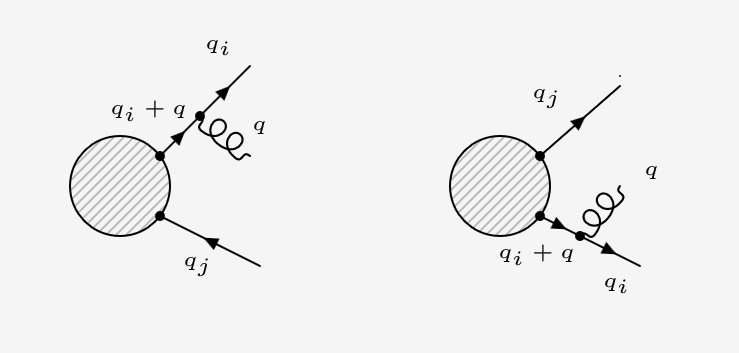
\includegraphics[width=0.85\textwidth]{images/qqg-diagrams.png}
\end{figure}

\subsection{qg-$\bar{q}$}

\begin{figure}[h!]
\centering
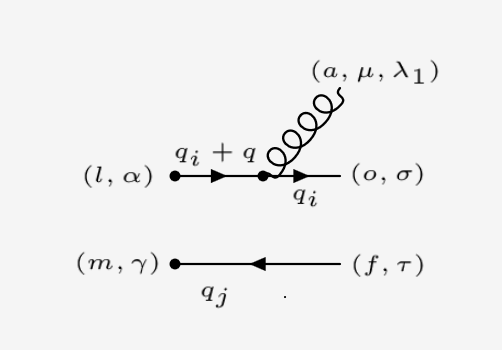
\includegraphics[width=0.85\textwidth]{images/qgqbarM.png}
\end{figure}


\begin{figure}[h!]
\centering
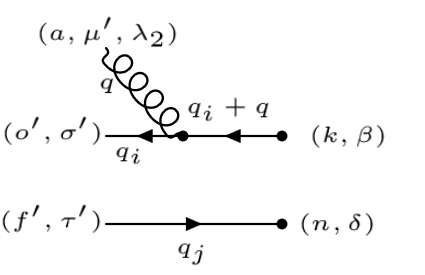
\includegraphics[width=0.85\textwidth]{images/qgqbarMDega.png}
\end{figure}


\begin{figure}[h!]
\centering
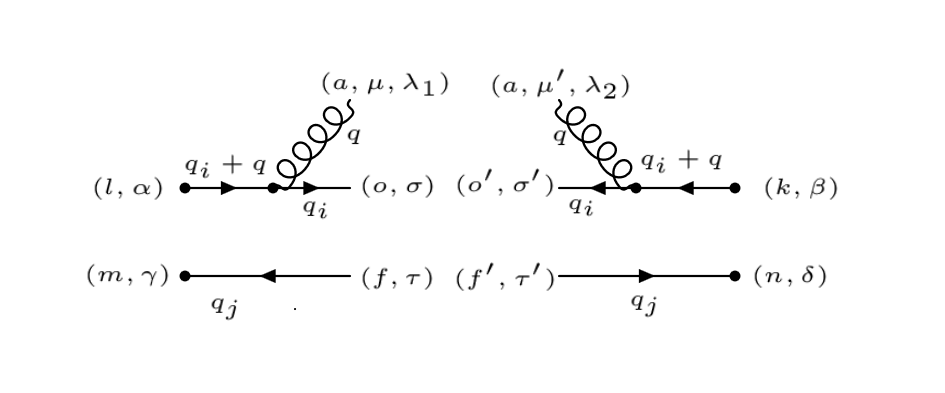
\includegraphics[width=0.85\textwidth]{images/qgqbarMSquer.png}
\end{figure}
\newpage

\subsection{$\bar{q}$g-q}

\begin{figure}[h!]
\centering
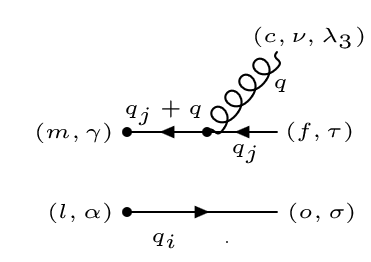
\includegraphics[width=0.85\textwidth]{images/qbargqM.png}
\end{figure}


\begin{figure}[h!]
\centering
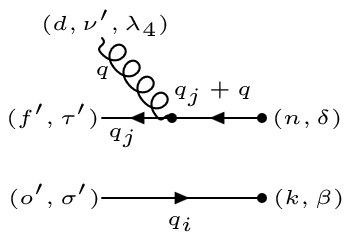
\includegraphics[width=0.85\textwidth]{images/qbargqMDega.png}
\end{figure}


\begin{figure}[h!]
\centering
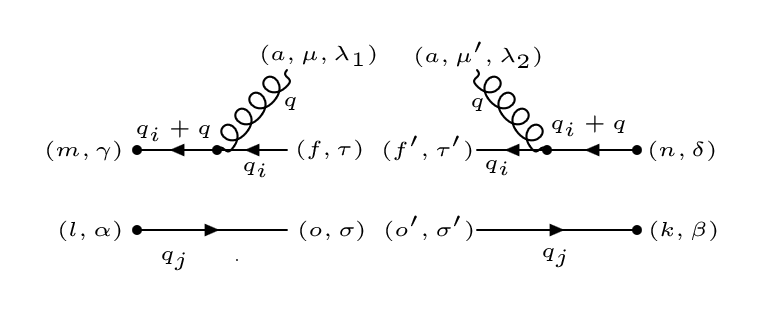
\includegraphics[width=0.85\textwidth]{images/qbargqMSquer.png}
\end{figure}
\newpage

\subsection{$M_1 {M_2}^{\dagger}$}

\begin{figure}[h!]
\centering
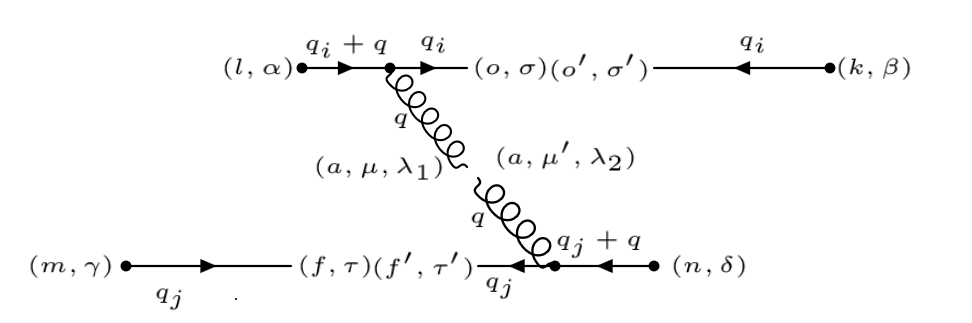
\includegraphics[width=0.85\textwidth]{images/M1M2Degaqqg.png}
\end{figure}

\subsection{$|M^{2}|$}

\begin{figure}[h!]
\centering
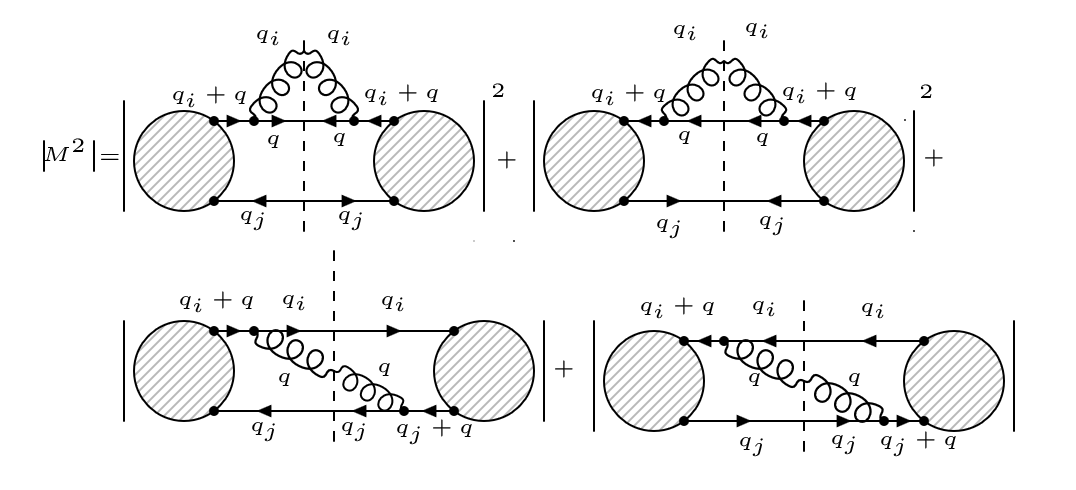
\includegraphics[width=0.85\textwidth]{images/qqgMSquer.png}
\end{figure}

\begin{figure}[h!]
\centering
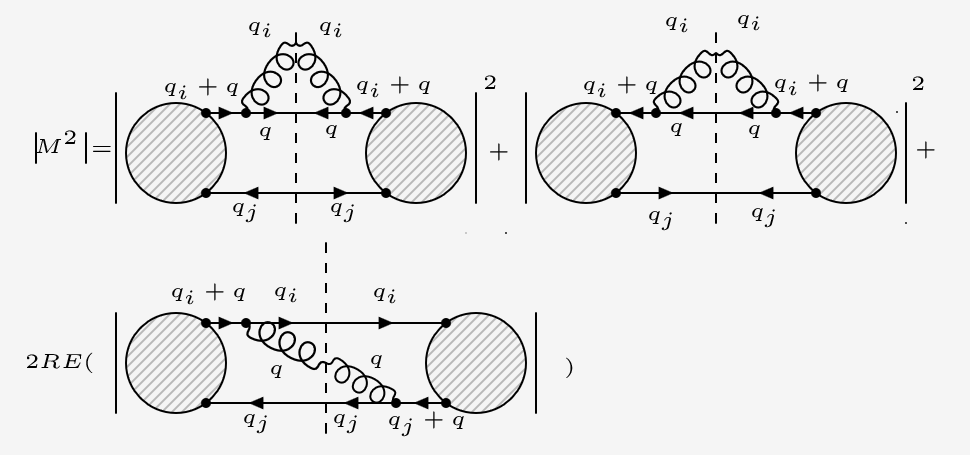
\includegraphics[width=0.85\textwidth]{images/REqqgMSquer.png}
\end{figure}

\newpage